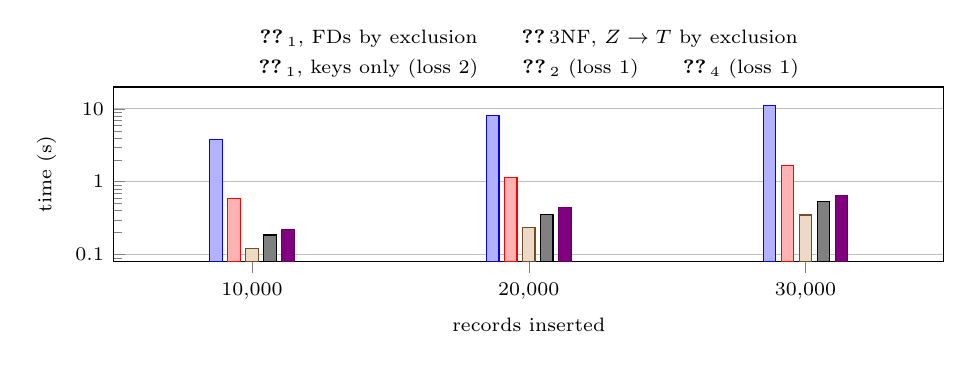
\begin{tikzpicture}
\begin{axis}[name=teaseraxis, ybar, width=\columnwidth, height=3.8cm, bar width=4.5pt, enlarge x limits=0.25,
  ylabel={time (s)}, xlabel={records inserted}, symbolic x coords={{10,000},{20,000},{30,000}}, xtick=data,
  ymode=log, log origin y=infty, ymin=0.08, ymax=20, log ticks with fixed point, tick pos=left,
  legend image code/.code={\draw[#1] (0cm,-0.07cm) rectangle (0.32cm,0.07cm);},
  tick label style={font=\scriptsize}, label style={font=\scriptsize}, ymajorgrids]
\addplot coordinates {({10,000},3.811) ({20,000},8.064) ({30,000},10.976)};
\label{plot:teaser-d1x}
\addplot coordinates {({10,000},0.582) ({20,000},1.150) ({30,000},1.673)};
\label{plot:teaser-3nfx}
\addplot coordinates {({10,000},0.121) ({20,000},0.235) ({30,000},0.350)};
\label{plot:teaser-d1}
\addplot coordinates {({10,000},0.186) ({20,000},0.352) ({30,000},0.531)};
\label{plot:teaser-d2}
\addplot coordinates {({10,000},0.223) ({20,000},0.440) ({30,000},0.656)};
\label{plot:teaser-d4}
\end{axis}
% two legend rows, each centered over the plot box (the y label is not counted): the designs with exclusion constraints, then the designs with keys only
\node[anchor=south, font=\scriptsize, inner sep=1pt] at ([yshift=13pt]teaseraxis.north) {\ref{plot:teaser-d1x}\,$\dec_1$, FDs by exclusion\qquad\ref{plot:teaser-3nfx}\,3NF, $Z\rightarrow T$ by exclusion};
\node[anchor=south, font=\scriptsize, inner sep=1pt] at ([yshift=2pt]teaseraxis.north) {\ref{plot:teaser-d1}\,$\dec_1$, keys only (loss 2)\qquad\ref{plot:teaser-d2}\,$\dec_2$ (loss 1)\qquad\ref{plot:teaser-d4}\,$\dec_4$ (loss 1)};
\end{tikzpicture}
